\chapter{Least-Square Approximation}

\section{Mathematical Ideas of Least-Square Approximation}

As discussed in Chapter \ref{chap:SolLinSys}, given a linear system $A\vec{x} = \vec{h}$, if the number of equations (rows) is greater than the number of unknowns (columns), then it is overdetermined. Generally, it would be inconsistent and no $\vec{x}$ can satisfy $A\vec{x} = \vec{h}$. However, a best-fit vector $\vec{x_f}$ can be found such that $A\vec{x_f} = \vec{h_f}$, the least-square error can be achieved in the sense that $\vec{h_f}$ has the closest distance to $\vec{h}$, i.e. the magnitude of the error vector $\vec{h}-\vec{h_f} = \vec{h}-A\vec{x_f}$ is minimized.\\
\\
It is stated that the desired vector $\vec{h_f} = A\vec{x_f}$ is the orthogonal projection of $\vec{h}$ onto the column space formed by column vectors in $A$. A simple description of column space can be found in Definition \ref{columnspace}. Intuitively, from a geometric viewpoint, $\vec{h_f} = A\vec{x_f}$ lies in the column space of $A$, and it would achieve the shortest distance to $\vec{h}$ if $\vec{h}-\vec{h_f}$ is orthogonal to column space of $A$. This also means that $A\vec{x} = \vec{h}$ has an exact solution if and only if $\vec{h}$ already lies in the column space of $A$.
\begin{center}
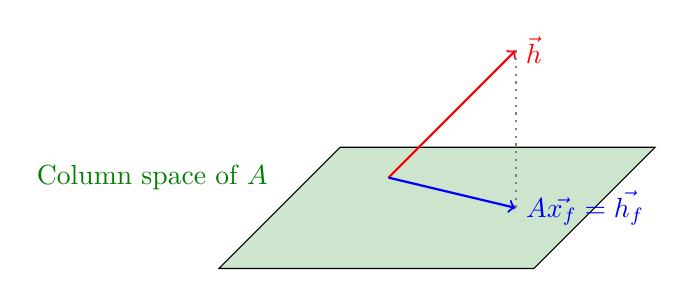
\begin{tikzpicture}
\filldraw[fill=Green!20]
(0,0,0) -- (4,0,0) -- (4,0,4) -- (0,0,4) -- cycle;
\draw[red, thick, ->] (1,0,1) -- (3,2,2) node[right]{$\vec{h}$};
\draw[blue, thick, ->] (1,0,1) -- (3,0,2) node[right]{$A\vec{x_f} = \vec{h_f}$};
\draw[gray, thick, dotted] (3,2,2) -- (3,0,2);
\node[Green] at (-2,0,1) {Column space of $A$};
\end{tikzpicture} \\
Geometric situation for the least-square approximation problem, when $A$ has 3 rows and 2 columns, $\vec{x_f}$ is a two-dimensional vector, while $\vec{h}$ and the orthogonal projection of $\vec{h}$ onto the column space of $A$, that is, $A\vec{x_f} = \vec{h_f}$ are three-dimensional vectors.
\end{center}

The remaining problem is to find either $\vec{h_f}$ or $\vec{x_f}$. Since the best-fit vector $\vec{h}-\vec{h_f}$ has to be orthogonal to all column vectors in $A$, $A^T(\vec{h}-\vec{h_f}) = \vec{0}$, as the dot products of rows in $A^T$ (columns in A) and $\vec{h}-\vec{h_f}$ evaluates to zero. Substitution and rearrangement gives
\begin{align*}
A^T(\vec{h}-\vec{h_f}) &= \vec{0} \\
A^T(\vec{h}-A\vec{x_f}) &= \vec{0} \\
A^T\vec{h} - A^TA\vec{x_f} &= \vec{0} \\
A^TA\vec{x_f} &= A^T\vec{h}
\end{align*}
This is called the normal equation due to the appearance of $A^TA$. Therefore,
\begin{align*}
\vec{x_f} &= (A^TA)^{-1}A^T\vec{h} \\  
\vec{h_f} &= A\vec{x_f} = A(A^TA)^{-1}A^T\vec{h}
\end{align*}
provided that the normal matrix $A^T A$ is invertible, which happens when $A$ consists of linearly independent column vectors.
\begin{thm}
\label{bestfit}
If $A$ is a $m \times n$ matrix with $m > n$ and all $n$ column vectors being linearly independent, then for the system $A\vec{x} = \vec{h}$, there exists a unique best-fit solution
\begin{align*}
\vec{x_f} &= (A^TA)^{-1}A^T\vec{h}    
\end{align*}
such that $\norm{\vec{h}-\vec{h_f}}^2 = \norm{\vec{h}-A\vec{x_f}}^2$ is minimized.
\end{thm}
However, if the column vectors in $A$ are not linearly independent, then the best-fit solution will not be unique. Rather, the normal equation will still be consistent, but there are infinitely many possible solutions, each having the same least-square error.\\
\\
Also, if we by chance have the QR decomposition of $A$, then
\begin{align*}
\vec{x_f} &= ((QR)^T(QR))^{-1}(QR)^T\vec{h} \\
&= (R^TQ^TQR)^{-1} (QR)^T\vec{h} \\
&= (R^TR)^{-1} R^TQ^T \vec{h} \\
&= R^{-1} (R^T){-1} R^TQ^T \vec{h} \\
&= R^{-1} Q^T\vec{h}
\end{align*}
$Q^TQ = I$ since $Q$ is orthogonal matrix as column vectors of $Q$ are orthonormal basis.

\section{Linear Regression}
\subsection{Linear Regression for One Predictor Variable}

Linear regression is a good example of least-square approximation. The simplest type of linear regression is fitting a straight line $y = \alpha + \beta x$ to $n$ pairs of observation, $(x_1, y_1), (x_2, y_2), \cdots, (x_n, y_n)$ such that the sum of squares error $\sum_{k=1}^n (y_k - (\alpha + \beta x_k))^2$ is minimized, optimizing the prediction of $y$ by $x$.

\begin{center}
\begin{tikzpicture}
\draw[thick, ->] (-1,0) -- (5,0) node[right]{$x$};
\draw[thick, ->] (0,-1) -- (0,5) node[above]{$y$};
\node[circle, inner sep=1pt, fill=blue] at (1,1.2) {};
\node at (0.8,1.6) {$(1,1.2)$};
\node[circle, inner sep=1pt, fill=blue] at (2,1.6) {};
\node at (2.2,1.2) {$(2,1.6)$};
\node[circle, inner sep=1pt, fill=blue] at (3,2.8) {};
\node at (3.2,2.4) {$(3,2.8)$};
\node[circle, inner sep=1pt, fill=blue] at (4,4.4) {};
\node at (3.8,4.8) {$(4,4.4)$};
\draw[thick, red] (-0.5,-0.74) -- (5,5.2) node[right]{$y = -0.2+1.08x$};
\node[below left]{$O$}; 
\draw[thick, Green] (1,1.2) -- (1,0.88);
\draw[thick, Green] (2,1.6) -- (2,1.96);
\draw[thick, Green] (3,2.8) -- (3,3.04);
\draw[thick, Green] (4,4.4) -- (4,4.12);
\end{tikzpicture}\\
Linear Regression for 4 data points. The red straight line represents the best linear fit, and the green lines are the distance, or errors between the actual data and the regression line, whose sum of square is minimized.
\end{center}

To see how we can apply the results in the last section, we first rewrite the system into matrix form. The actual values are given by $\vec{y}^T = (y_1, y_2, \cdots, y_n)$, while the fitted values will be in the form of $(\alpha\vec{1} + \beta \vec{x})^T = (\alpha + \beta x_1, \alpha + \beta x_2, \cdots, \alpha + \beta x_n)^T$, where $\vec{1}$ is a column vector filled with ones, $\alpha$ and $\beta$ are the intercept and slope to be determined.
In other words, we are trying to find the best-fit for the system
\begin{align*}
\alpha\vec{1} + \beta \vec{x} &= \vec{y}
\end{align*}
or alternatively
\begin{align*}
\begin{bmatrix}
1 & x_1 \\
1 & x_2 \\
\vdots & \vdots \\
1 & x_n
\end{bmatrix}
\begin{bmatrix}
\alpha \\
\beta
\end{bmatrix}
=
\begin{bmatrix}
y_1 \\
y_2 \\
\vdots \\
y_n
\end{bmatrix}
\end{align*}
Usually we will denote such system as $[X]\vec{\beta} = \vec{y}$, where the first and second column of $[X] = [\vec{1}|\vec{x}]$ represent two predictor variables. Specifically, the first predictor is the constant term and represents the $y$-intercept. Now, the sum of square errors $\sum_{k=1}^n (y_k - (\alpha + \beta x_k))^2 = \norm{\vec{y} - [X]\vec{\beta}}^2$, is minimized by the best-fit parameters
\begin{align*}
\vec{\beta_f} = ([X]^T[X])^{-1}[X]^T \vec{y}
\end{align*}
according to Theorem \ref{bestfit}. Expanding the expression, the parameters for single variable linear regression are
\begin{align*}
\begin{bmatrix}
\alpha_f \\
\beta_f
\end{bmatrix}
& =
\left(
\begin{bmatrix}
1 & 1 & \cdots & 1 \\
x_1 & x_2 & \cdots & x_n
\end{bmatrix}
\begin{bmatrix}
1 & x_1 \\
1 & x_2 \\
\vdots & \vdots \\
1 & x_n
\end{bmatrix} 
\right)^{-1}
\begin{bmatrix}
1 & 1 & \cdots & 1 \\
x_1 & x_2 & \cdots & x_n
\end{bmatrix}
\begin{bmatrix}
y_1 \\
y_2 \\
\vdots \\
y_n
\end{bmatrix} \\
&= 
\begin{bmatrix}
n & \sum X \\
\sum X & \sum (X^2)
\end{bmatrix}^{-1}
\begin{bmatrix}
\sum Y \\
\sum (XY)
\end{bmatrix} \\
&=
\frac{1}{n\sum(X^2) - (\sum X)^2}
\begin{bmatrix}
\sum(X^2) & -\sum X \\
-\sum X & n
\end{bmatrix}
\begin{bmatrix}
\sum Y \\
\sum (XY)
\end{bmatrix} \\
&=
\frac{1}{n\sum(X^2) - (\sum X)^2}
\begin{bmatrix}
\sum Y \sum (X^2) - \sum X \sum (XY) \\
n \sum(XY) - \sum X \sum Y
\end{bmatrix}
\end{align*}
where we have used the results in Example \ref{ex2.3.3} to calculate the inverse.
\begin{proper}
\label{bestfit2}
The best-fit parameters for single predictor variable linear regression are
\begin{align*}
\alpha_f &= \frac{\sum Y \sum (X^2) - \sum X \sum (XY)}{n\sum(X^2) - (\sum X)^2} \\
\beta_f &= \frac{n \sum(XY) - \sum X \sum Y}{n\sum(X^2) - (\sum X)^2}
\end{align*}
such that the regression line $y = \alpha + \beta x$ achieves the least-square error.
\end{proper}
\begin{exmp}
\label{ex11.1.1}
Find the best linear fit for five $(x,y)$ data points, which are $(2,4)$, $(3,6)$, $(4,7)$, $(5,9)$, $(7,11)$.\\
\\
We first compute the following quantities
\begin{align*}
\sum X &= 2+3+4+5+7 = 21 \\
\sum(X^2) &= 2^2+3^2+4^2+5^2+7^2 = 103 \\
\sum Y &= 4+6+7+9+11 = 37 \\
\sum (XY) &= (2)(4)+(3)(6)+(4)(7)+(5)(9)+(7)(11) = 176
\end{align*}
With $n=5$, using Properties \ref{bestfit2}, the required parameters are
\begin{align*}
\alpha_f &= \frac{\sum Y \sum (X^2) - \sum X \sum (XY)}{n\sum(X^2) - (\sum X)^2} = \frac{(37)(103)-(21)(176)}{(5)(103)-(21)^2} \approx 1.554 \\
\beta_f &= \frac{n \sum(XY) - \sum X \sum Y}{n\sum(X^2) - (\sum X)^2} = \frac{(5)(176)-(21)(37)}{(5)(103)-(21)^2} \approx 1.392
\end{align*}
So the best linear fit is around $y = 1.554 + 1.392x$.
\end{exmp}

\subsection{Linear Regression for Multiple Predictor Variables}

Sometimes we may need to predict a variable $y$ with multiple predictor variables $x^{(1)}, x^{(2)}, \cdots$ as different variables are often interlinked in Earth Science scenario. We can extend the earlier results, where Theorem \ref{bestfit} is still applicable. Linear regression for multiple predictor variables will produce a best fit equation in the form of $y = \alpha + \beta_1x^{(1)} + \beta_2x^{(2)} + \cdots$. The computation of the parameters use the same formula
\begin{align*}
\vec{\beta_f} = ([X]^T[X])^{-1}[X]^T \vec{y}
\end{align*}
where in this case the quantities extend to include more predictor variables, $\vec{\beta_f}^T = (\alpha_f, {\beta_1}_f, {\beta_2}_f, \cdots)^T$, and the matrix $[X] = [\vec{1}|\vec{x}^{(1)}|\vec{x}^{(2)}|\cdots]$ holds the observed predictor variables column by column.

\begin{exmp}
Find a quadratic fit for Example \ref{ex11.1.1}.\\
\\
The predictor variables are the constant term, $x$, as well as $x^2$. The desired parameters are
\begin{align*}
\vec{\beta_f} &= ([X]^T[X])^{-1}[X]^T \vec{y} \\
&=
\left(
\begin{bmatrix}
1 & 1 & 1 & 1 & 1 \\
2 & 3 & 4 & 5 & 7 \\
2^2 & 3^2 & 4^2 & 5^2 & 7^2
\end{bmatrix}
\begin{bmatrix}
1 & 2 & 2^2 \\
1 & 3 & 3^2 \\
1 & 4 & 4^2 \\
1 & 5 & 5^2 \\
1 & 7 & 7^2 
\end{bmatrix}
\right)^{-1}
\begin{bmatrix}
1 & 1 & 1 & 1 & 1 \\
2 & 3 & 4 & 5 & 7 \\
2^2 & 3^2 & 4^2 & 5^2 & 7^2
\end{bmatrix}
\begin{bmatrix}
4 \\
6 \\
7 \\
9 \\
11
\end{bmatrix} \\
& \approx
\begin{bmatrix}
-0.009 \\
2.201 \\
-0.089 
\end{bmatrix}
\end{align*}
The quadratic fit is thus $y = -0.089 + 2.201x - 0.089x^2$.
\end{exmp}
Usually, fitting a degree $p$ polynomials to $n$ points, $p \leq n$, will involve a matrix in the form
\begin{align*}
[X]
&= 
\begin{bmatrix}
1 & x_1 & x_1^2 & \cdots & x_1^p \\
1 & x_2 & x_2^2 & \cdots & x_2^p \\
\vdots & \vdots & \vdots & & \vdots \\
1 & x_n & x_n^2 & \cdots & x_n^p \\
\end{bmatrix} 
\end{align*}
This class of matrices is called Vandermonde matrices.\\
\\
Before going to the next topic, we derive some features of linear regression. The errors, or called the residuals $e_i = h_i - (h_i)_f$, have a mean of zero. Using matrix notation, it means that the sum of elements in the vector $\vec{e} = \vec{h} - \vec{h_f}$ is zero. This can be seen from the very beginning of our derivation for the best fit problem $A\vec{x} = \vec{h}$, where the condition has been $A^T(\vec{h} - \vec{h}_f) = \vec{0}$. For linear regression, it becomes $[X]^T\vec{e} = \vec{0}$. However, since one column in $[X]$ is $\vec{1}$, one of the elements in $[X]^T\vec{e}$ is just $\vec{1} \cdot \vec{e}$, which is just the sum of errors. As $[X]^T\vec{e} = \vec{0}$, the sum and hence the mean of errors must be zero.\\
\\
Another property is that, if we denote the mean of $y$ as $\bar{y}$, each actual data and predicted values as $y_i$ and $\hat{y_i}$, then
\begin{align*}
\sum_i (y_i - \overline{y})^2 &= \sum_i (y_i - \hat{y}_i)^2 + \sum_i (\hat{y}_i - \overline{y})^2
\end{align*}
The term at the left hand side is SST/Sum of Squares Total, while the two terms at the right hand side are SSE/Sum of Squares Error and SSR/Sum of Squares Regression. To prove this, we expand the SST, which gives
\begin{align*}
\text{SST} &= \sum_i (y_i - \overline{y})^2 \\
&= \sum_i ((y_i - \hat{y}_i) + (\hat{y}_i - \overline{y}))^2 \\
&= \sum_i (y_i - \hat{y}_i)^2 + \sum_i (\hat{y}_i - \overline{y})^2 + 2\sum_i ((y_i - \hat{y}_i) (\hat{y}_i - \overline{y})) \\
&= \text{SSE} + \text{SSR} + 2\sum_i ((y_i - \hat{y}_i) (\hat{y}_i - \overline{y}))
\end{align*}
The remaining task is to prove that the last term equals to zero. For simplicity, we work with single predictor variable so there are two parameters $\alpha$ and $\beta$ only. Expanding the product gives
\begin{align*}
\sum_i ((y_i - \hat{y}_i) (\hat{y}_i - \overline{y})) &= \sum_i (\hat{y}_i(y_i - \hat{y}_i)) - \overline{y} \sum_i (y_i - \hat{y}_i) \\
&= \sum_i ((\alpha + \beta x_i)(y_i - \hat{y}_i)) - \overline{y} \sum_i (y_i - \hat{y}_i) \\
&= \beta \sum_i (x_i(y_i - \hat{y}_i)) - (\overline{y} - \alpha) \sum_i (y_i - \hat{y}_i) \\
&= \beta \sum_i (x_i e_i) - (\overline{y} - \alpha) \sum_i e_i
\end{align*}
Using the same logic as we have investigated $[X]^T\vec{e} = \vec{0}$ before, we know that
\begin{align*}
\vec{1} \cdot \vec{e} &= \sum_i e_i = 0 \\
\vec{x} \cdot \vec{e} &= \sum_i (x_i e_i) = 0
\end{align*}
These two equations can also be derived by setting $\partial (\sum_i e_i^2)/\partial \alpha = \partial (\sum_i e_i^2)/\partial \beta = 0$ as the sum of squares error reaches minimum at the point of best fit. Substituting this two equations implies that $\sum_i ((y_i - \hat{y}_i) (\hat{y}_i - \overline{y})) = 0$, and thus $\text{SST} = \text{SSE} + \text{SSR}$. We repeat these two results as follows.
\begin{proper}
Linear Regression has the properties that the mean error is zero, and sum of squares total is equal to sum of squares error plus sum of squares regression.
\end{proper}
$R^2$, which is the ratio of SSR to SST, indicates how well the regression is. If $R^2$ is close to one, then the fit is usually good, unless it is overfitted. However, if $R^2$ is close to zero, the regression is useless.


\section{Exercise}

\begin{Exercise}
Find a linear fit for the following data about sea level pressure and temperature measured at a weather station.
\begin{center}
\begin{tabular}{|c|c|c|c|c|c|c|}
\hline
Temperature (deg C) & 10 & 12 & 12 & 13 & 16 & 17\\
\hline
Pressure (hPa) & 1022 & 1019 & 1018 & 1017 & 1014 & 1013\\
\hline
\end{tabular}
\end{center}
\end{Exercise}

\begin{Exercise}
Find a linear fit and a quadratic fit for the following atmospheric data regarding global carbon dioxide level. Also, calculate the root mean square error for each fit.
\begin{center}
\fbox{\includegraphics[scale = 0.3]{carbon.png}}
\end{center}
\begin{center}
\begin{tabular}{|c|c|c|c|c|c|c|}
\hline
Years passed since 1960 & 0 & 5 & 10 & 15 & 20 & 25 \\
\hline
$CO_2$ level (ppm) & 317 & 320 & 326 & 331 & 339 & 346 \\
\hline
Years passed since 1960 & 30 & 35 & 40 & 45 & 50 & 55\\
\hline
$CO_2$ level (ppm) & 354 & 361 & 370 & 380 & 390 & 401\\
\hline
\end{tabular}
\end{center}
(Data from: \href{ftp://aftp.cmdl.noaa.gov/products/trends/co2/co2_annmean_mlo.txt}{NOAA})
\end{Exercise}

\begin{Exercise}
Radioactive decay is modelled by $N = N_0e^{-kt}$, where $N_0$ and $k$ are the initial concentration and the decay constant respectively. While the expression is exponential, not linear, the technique of linear fit can still be applied if the data undergoes linearization. Show that by the substitution $n = \ln N$ the equation can be transformed into a linear equation $n = \ln N = \ln N_0 - kt = n_0 - kt$. Hence find the best linear fit on $(t, n)$ by finding the parameters $(n_0, k)$ from the experimental data on the radioactive isotope Sodium-24 below and recover the decay constant and initial mass.
\begin{center}
\begin{tabular}{|c|c|c|c|c|c|c|}
\hline
Time passed (hr) & 6 & 8 & 12 & 24 & 36 & 48\\
\hline
Mass (g) & 75.8 & 69.1 & 57.3 & 33.0 & 18.8 & 10.8\\
\hline
\end{tabular}
\end{center}
\end{Exercise}

